\documentclass[12pt]{article}

\usepackage{amsmath}
\usepackage{amsfonts}
\usepackage{float}
\usepackage{fancyhdr}
\usepackage{graphicx}
\usepackage[colorlinks=true,linkcolor=blue, citecolor=red]{hyperref}
\usepackage{url}
\usepackage[top=.75in, left=.5in, right=.5in, bottom=1in]{geometry}
\usepackage{parskip}
\usepackage{tabularx}
\usepackage[utf8]{vietnam}
\usepackage{multicol}
\usepackage{tikz}

\usetikzlibrary{calc,trees,positioning,arrows.meta,chains,shapes.geometric, decorations.pathreplacing,decorations.pathmorphing,shapes, matrix,shapes.symbols, fit}
\tikzset{
    every node/.style={
        font=\scriptsize
    },
    decision/.style={
        shape=rectangle,
        minimum height=1cm,
        text width=2cm,
        text centered,
        rounded corners=1ex,
        draw,
        label={[yshift=0.125cm]left:yes},
        label={[yshift=0.125cm]right:no},
    },
    outcome/.style={
        shape=ellipse,
        fill=gray!15,
        draw,
        text width=1.5cm,
        text centered
    },
    decision tree/.style={
        edge from parent path={[-latex] (\tikzparentnode) -| (\tikzchildnode)},
        sibling distance=3cm,
        level distance=1.125cm
    }
}
\tikzstyle{block} = [rectangle, draw, text centered, rounded corners, minimum height=3em]

\setlength{\headheight}{29.43912pt}

\pagestyle{fancy}
\lhead{
Báo cáo Đồ án môn học
}
\rhead{
Trường Đại học Khoa học Tự nhiên - ĐHQG HCM\\
\coursename
}
\lfoot{\LaTeX\ by \href{https://github.com/trhgquan}{Quan, Tran Hoang}}

\newcommand{\coursename}{CSC15008 - Xử lý ngôn ngữ tự nhiên ứng dụng}
\newcommand{\reportname}{Ứng dụng Decision Tree xây dựng công cụ Fakenews Detection}

\begin{document}

\begin{titlepage}
\newcommand{\HRule}{\rule{\linewidth}{0.5mm}}
\centering

\textsc{\LARGE đại học quốc gia tphcm}\\[1.5cm]
\textsc{\Large trường đại học khoa học tự nhiên}\\[0.5cm]
\textsc{\large khoa công nghệ thông tin}\\[0.5cm]
\textsc{bộ môn công nghệ tri thức}\\[0.5cm]

\HRule \\[0.4cm]
{ 
\huge{\bfseries{Báo cáo Đồ án môn học}}\\[0.5cm]
\large{\bfseries{Đề tài: \reportname}}
}\\[0.4cm]
\HRule \\[0.5cm]

\textbf{\large Môn học: \coursename}\\[0.5cm]

\begin{minipage}[t]{0.4\textwidth}
\begin{flushleft} \large
\emph{Sinh viên thực hiện:}\\
Trần Hoàng Quân (19120338)\\
Lê Hoàng Trọng Tín \textsc{(19120682)}
\end{flushleft}
\end{minipage}
~
\begin{minipage}[t]{0.4\textwidth}
\begin{flushright} \large
\emph{Giáo viên hướng dẫn:} \\
% Dr. James \textsc{Smith}
Thầy Nguyễn Hồng Bửu Long
\end{flushright}
\end{minipage}\\[2cm]

{\large \today}\\[2cm]

\includegraphics[scale=.25]{img/hcmus-logo.png}\\[1cm] 

\vfill
\end{titlepage}
	
	
\tableofcontents
\pagebreak

\section{Giới thiệu đề tài}
\subsection{Tổng quan bài toán Text Classification (Phân loại văn bản)}
\begin{figure}[H]
	\centering
	\begin{tikzpicture}
		[node distance=4cm,
		start chain=going right,]
		\node (n1) at (0,0) [block]  {Document};
		\node (n2) [block, right of=n1] {Feature Extraction};
		\node (n3) [block, right of=n2] {Classification Model};
		\node (n4) [block, right of=n3] {Evaluation};
		\node (n5) at (6,2) [block] {Dimensionality Reduction};
		% Connectors
		\draw [->] (n1) -- (n2);
		\draw [->, dashed] (n2) -- (n3);
		\draw [->] (n3) -- (n4);
		\draw[->, dashed, to path={-| (\tikztotarget)}](n5) edge (n3);
		\draw[->, dashed, to path={|- (\tikztotarget)}](n2) edge (n5);
	\end{tikzpicture}
	\caption{Tổng quan bài toán Text Classification (Phân loại văn bản)\cite{Kowsari_2019}}
\end{figure}
\begin{itemize}
\item Document: ngữ liệu có thể là văn bản, đoạn văn (paragraph), câu văn (sentence) hoặc một phần của câu (sub-sentence).
\item Feature Extraction: trích xuất các đặc trưng từ ngữ liệu.
\item Dimensionality Reduction: làm giảm số lượng đặc trưng, qua đó làm giảm chi phí tính toán và bộ nhớ sử dụng.
\item Classificaion Model: có thể là một hoặc nhiều classifier (bộ phân lớp) kết hợp để phân loại ngữ liệu.
\item Evaluation: Prediction và Scoring, đánh giá mô hình dựa trên kết quả phân loại.
\end{itemize}

\subsection{Đề tài Fakenews Detection (Phân loại tin giả)}
Tin giả (fake news) đã trở thành mối quan tâm trong những năm gần đây. Nhiều hệ thống phân loại tin giả đã được xây dựng và hoạt động rất tốt, dựa trên các mô hình học máy phổ biến.

Dựa trên mô hình Cây quyết định (Decision Tree) và một số mô hình học máy khác, nhóm tạo ra một công cụ phân loại tin giả, cho kết quả chính xác ở mức chấp nhận được. Dù kết hợp nhiều mô hình học máy nhưng trọng tâm của nhóm sẽ tìm hiểu, nghiên cứu và phát triển xoay quanh mô hinh Cây quyết định.
\section{Quá trình xây dựng công cụ}
\subsection{Dữ liệu}
Dữ liệu lấy từ Kaggle gồm 44898 bài báo, trích từ các nền tảng nổi tiếng trong năm 2017. \href{https://www.kaggle.com/datasets/clmentbisaillon/fake-and-real-news-dataset}{Đường link đến dataset}.

\subsection{Tiền xử lý (Preprocessing)}
Các bước tiền xử lí bao gồm:
\begin{itemize}
\item Chuyển câu về dạng chữ thường
\item Loại bỏ dấu câu
\item Loại bỏ số, vì số liệu thường gây "nhiễu" trong quá trình phân loại.
\item Loại bỏ hyperlinks, html tags và các kí tự đặc biệt.
\item Loại bỏ stopwords, trong trường hợp này là stopwords tiếng Anh.
\item Thêm class để nhận biết tin thật và tin giả.
\end{itemize}
\begin{figure}[H]
    \centering
    \includegraphics[scale=.8]{img/data-summerise.png}
    \caption{Tương quan các lớp fake (0) và real (1) trong dataset}
    \label{fig:real_fake_in_train}
\end{figure}

\subsection{Trích xuất đặc trưng (Feature Extraction)}
Ta không tiến hành "học thuộc" một câu, mà chỉ học các đặc trưng của câu đó. Có nhiều phương pháp trích xuất đặc trưng: Bag of Words (BoW), TF-IDF, GloVe, Word2Vec, ..etc.

Một ví dụ: Với câu văn \textit{The quick brown fox jumps over the lazy dog}, các features được trích xuất với TF-IDF là \{brown, dog, fox, jumps, lazy, quick\}.
\subsubsection{TF-IDF (Term Frequency - Inverse Document Frequency)}
Đươc Karen Spärck Jones sáng chế năm 1972\cite{Jones72astatistical}, phương pháp này làm giảm ảnh hưởng những từ thường xuyên xuất hiện trong corpus. Trọng số $W$ của một từ (term) $t$ trong văn bản (document) $d$ được tính như sau:
$$
W(d, t) = TF(d, t) \times \log\left(\frac{N}{df(t)}\right)
$$
Với $N$ là tổng số document, $df(t)$ là tổng số lượng document chứa term $t$, $TF(d, t)$ là số lần xuất hiện của từ $t$ trong document $d$.

\subsection{Cây quyết định (Decision Tree)}
Thuật toán phân lớp sử dụng Cây quyết định (Decision Tree) được Ross Quinlann phát minh năm 1986\cite{DBLP:journals/ml/Quinlan86}, là phương pháp xuất hiện từ rất sớm và rất thành công trong nhiều lĩnh vực của Học máy nói chung và Text Classification nói riêng. Từ 1986 đến nay đã có các phiên bản ID3, ID4.5, ID5.0, CART.\footnote{\texttt{sklearn.tree.DecisionTreeClassifier} sử dụng phiên bản customise của thuật toán CART.\cite{scikit-learn}}

Ý tưởng của thuật toán là tạo một cấu trúc dữ liệu cây, mỗi nút lá là một thuộc tính của tập dữ liệu đã phân lớp; mỗi nút không phải nút lá biểu thị một phép thử với một thuộc tính; mỗi nhánh biểu thị kết quả của phép thử. Ví dụ một cây quyết định và tập dữ liệu phân lớp:
\begin{figure}[H]
\begin{multicols}{2}
\begin{tikzpicture}
\node [decision] { Hết kem đánh răng? }
[decision tree]
child { node [decision] { Trời đang mưa? }
    child { node [outcome] { Ở nhà } }
    child { node [outcome] { Đi mua } }
}
child { node [outcome] { Ở nhà } };
\end{tikzpicture}

\begin{tabular}{|l|l|l|}
	\hline
	Hết kem đánh răng & Trời mưa & Quyết định \\
	\hline
	Có & Có & Ở nhà \\
	Có & Không & Đi mua \\
	Không & Có & Ở nhà \\
	Không & Không & Ở nhà \\
	\hline
\end{tabular}
\end{multicols}
\caption{Ví dụ một cây quyết định và tập dữ liệu phân lớp}
\end{figure}
Để xác định đâu là nút cha, đâu là nút con, thuật toán tiến hành lựa chọn các đặc trưng (Feature Selection) dựa trên các độ đo \textbf{Information Gains} và \textbf{Gini Index}.

\subsubsection{Lựa chọn đặc trưng (Feature Selection) với độ đo Information Gains}
Gọi $\mathbf{p} = (p_1, p_2, .., p_n)$ là phân phối sao cho biến ngẫu nhiên $x$ nhận $n$ giá trị $(x_1, x_2, .., x_n)$ và xác suất lần lượt là $(p_1, p_2, .., p_n)$. Hàm số Entropy $H(\mathbf{p})$ được định nghĩa như sau:
$$
H(\mathbf{p}) = -\sum_{i = 1}^n p_i \log(p_i)
$$
Ví dụ: một tập dữ liệu có $p$ mẫu được gán nhãn \textit{positive} và $n$ mẫu được gán nhãn \textit{negative}. Khi đó entropy $H(\frac{p}{n + p}, \frac{n}{n + p})$ được tính như sau:
$$
H\left(\frac{p}{n + p}, \frac{n}{n + p}\right) = -\frac{p}{n + p}\log\left(\frac{p}{n + p}\right) - \frac{n}{n + p}\log\left(\frac{n}{n + p}\right)
$$
Chọn thuộc tính $A$ có $k$ giá trị khác nhau, chia tập train $E$ thành $k$ tập con $\{E_1, E_2, .., E_k\}$. \textbf{Entropy kỳ vọng (EH)} còn lại sau khi chọn $A$ là một nút được tính như sau:
$$
EH(A) = \sum_{i = 1}^{n}\left(\frac{p_i + n_i}{p + n}\right)H\left(\frac{p_i}{n_i + p_i}, \frac{n_i}{n_i + p_i}\right)
$$
Khi đó độ đo Information Gains của thuộc tính $A$ là hiệu của \textbf{Entropy} và \textbf{Entropy kỳ vọng}:
$$
A(I) = H\left(\frac{p}{n + p}, \frac{n}{n + p}\right) - EH(A) 
$$
Ta sẽ chọn thuộc tính nào có Information Gains lớn nhất làm nút cha.

\subsubsection{Lựa chọn đặc trưng (Feature Selection) với độ đo Gini Index}
Gini Index được tính toán như sau:
$$
\text{Gini} = 1 - \sum_{i = 1}^n p_i ^ 2
$$
Khác với Entropy, ta chọn thuộc tính có Gini Index nhỏ nhất làm nút cha, sau đó tính toán Gini Index với các nút còn lại.

\section{Huấn luyện, Kiểm thử và Triển khai}

\subsection{Huấn luyện \& Kiểm thử}
Tiến hành huấn luyện với các thông số sau:
\begin{itemize}
\item Kích thước training dataset: 44798 articles, đã gán nhãn.
\item Kích thước testing dataset: 100 articles, đã gán nhãn. Đây là 50 article chọn ngẫu nhiên từ tập True \& 50 article chọn ngẫu nhiên từ tập Fake.
\item Trích xuất đặc trưng: sử dụng \texttt{sklearn.feature\_extraction.text.TfidfVectorizer} với tham số \texttt{stop\_words = 'english'}. Tổng số đặc trưng trích xuất: 121613.
\item Bộ phân lớp: \texttt{sklearn.tree.DecisionTreeClassifier} với tham số \texttt{criterion = 'entropy'} 
\end{itemize}
\begin{figure}[H]
\begin{multicols}{2}
\includegraphics[scale=.5]{img/train-result.png}

\begin{table}[H]
\begin{tabular}{l l l l l}
\hline
 & precision & recall & f1-score & support \\
\hline
0 & 1.00 & 1.00 & 1.00 & 50 \\
1 & 1.00 & 1.00 & 1.00 & 50 \\
accuracy &   &   & 1.00 & 100 \\
macro avg & 1.00 & 1.00 & 1.00 & 100 \\
weighted avg & 1.00 & 1.00 & 1.00 & 100 \\
\hline
\end{tabular}
\end{table}
\end{multicols}
\label{fig:heatmap_testing}
\caption{Heatmap và \texttt{classification\_report} sau khi train}
\end{figure}
Như có thể thấy, độ chính xác của mô hình là gần như tuyệt đối (1.00).

\subsection{Pipeline}
Ngoài Decision Tree, ứng dụng có dùng một số mô hình khác: Logistic Regression, SGD, Random Forest, Gradient Boosting, k-Nearest Neighbors, Multinomial Naive Bayes và Linear SVM.

Kết quả dự đoán:
\begin{itemize}
	\item Nếu số lượng \textit{fake} predictions $\geq$ \textit{real} predictions, tin đó là tin \textbf{fake}.
	\item Nếu số lượng \textit{fake} predictions $<$ \textit{real} predictions, tin đó là tin \textbf{real}.
\end{itemize}
\begin{figure}[H]
	\centering
	\begin{tikzpicture}[
		node distance=7mm,
		title/.style={font=\fontsize{4}{4}\color{black!50}},
		typetag/.style={rectangle, draw=black!50, font=\scriptsize\ttfamily, anchor=west}
		]
		\node (dat) at (-5, -2.75) [draw=black!50, block] {Article};
		\node (pp) at (-3, -2.75) [draw=black!50, block] {Preprocess};
		
		\node (vt) at (-.5, -2.43) [title] {Vectorizer};
		\node (tf) [below=of vt.west, typetag, xshift=2mm] {TF-IDF};
		
		\node (vts) [draw=black!50, rounded corners, fit={(vt) (tf)}] {};
		
		\node (cl) at (2.5, 0) [title] {Classifier};
		
		\node (dt) [below=of cl.west, typetag, xshift=2mm] {Decision Tree};
		\node (lr) [below=of dt.west, typetag] {Logistic Regression};
		\node (sc) [below=of lr.west, typetag] {SGD};
		\node (rf) [below=of sc.west, typetag] {Random Forest};
		\node (gb) [below=of rf.west, typetag] {Gradient Boosting};
		\node (kn) [below=of gb.west, typetag] {K-Nearest Neighbors};
		\node (nb) [below=of kn.west, typetag] {Multinomial NB};
		\node (ls) [below=of nb.west, typetag] {Linear SVM};
		
		\node (cls) [draw=black!50, rounded corners, fit={(cl) (dt) (lr) (sc) (rf) (gb) (kn) (nb) (ls)}] {};
		
		\node (pred) at (7, -2.77) [draw=black!50, block] {Prediction};
		
		\draw [->] (dat) -- (pp);
		\draw [->] (pp) -- (vts);
		\draw [->] (vts) -- (cls);
		\draw [->] (cls) -- (pred);
	\end{tikzpicture}
	\caption{Fakenews Detection Pipeline}
\end{figure}

\subsection{Demo}
Ứng dụng sử dụng microframework Flask để deploy trên nền web. Giao diện sử dụng Bootstrap v5. Các bước cài đặt như sau:


\section{Tổng kết}
Một số ưu điểm có thể kể đến:
\begin{itemize}
\item Các thuật toán dùng trong đề tài là các thuật toán phổ biến, dễ cài đặt.
\item Cho độ chính xác cao với tập dữ liệu nhỏ.
\item Thời gian huấn luyện tương đối nhanh.
\end{itemize}
Tuy nhiên, đi kèm là một số khuyết điểm:
\begin{itemize}
\item Một số mô hình rất dễ bị overfit.
\item Xáo trộn dữ liệu có thể dẫn đến kết quả bị sai khác.\cite{Kowsari_2019}
\end{itemize}
Với sản phẩm hoàn chỉnh, bạn đọc có thể xem tại \href{https://github.com/trhgquan/fakenews-detection}{GitHub Repository}.

\cleardoublepage
\phantomsection
\addcontentsline{toc}{section}{Tài liệu}
\bibliographystyle{plain}
\bibliography{sample}

\end{document}